\clearpage{\pagestyle{empty}\cleardoublepage}

\chapter{The ATLAS experiment at the Large Hadron Collider}\label{chap:atlas}

The analyses presented in this dissertation have been performed analyzing data from 
proton-proton (p-p) collisions at the \cme $\rts=8\tev$ recorded during the year 2012 
at the ATLAS experiment~\cite{Aad:2008zzm}. In the following Chapter we will briefly 
describe the main features of the detector, located at the CERN laboratories in Geneva,
Switzerland.

The experimental facilities are situated at Point~1 along the Large Hadron Collider 
(LHC)~\cite{lhc} 27~km long ring, shown in Figure~\ref{fig:lhcring}. The accelerator
tunnel can reach an underground depth of 175~meters and is spread between Swiss
and French territory, while the cave where ATLAS is allocated is about 100~meters 
underground in the CERN Swiss site of Meyrin. 

\begin{figure}[tb]\begin{center}
	\subfigure{\label{fig:lhcring}
  	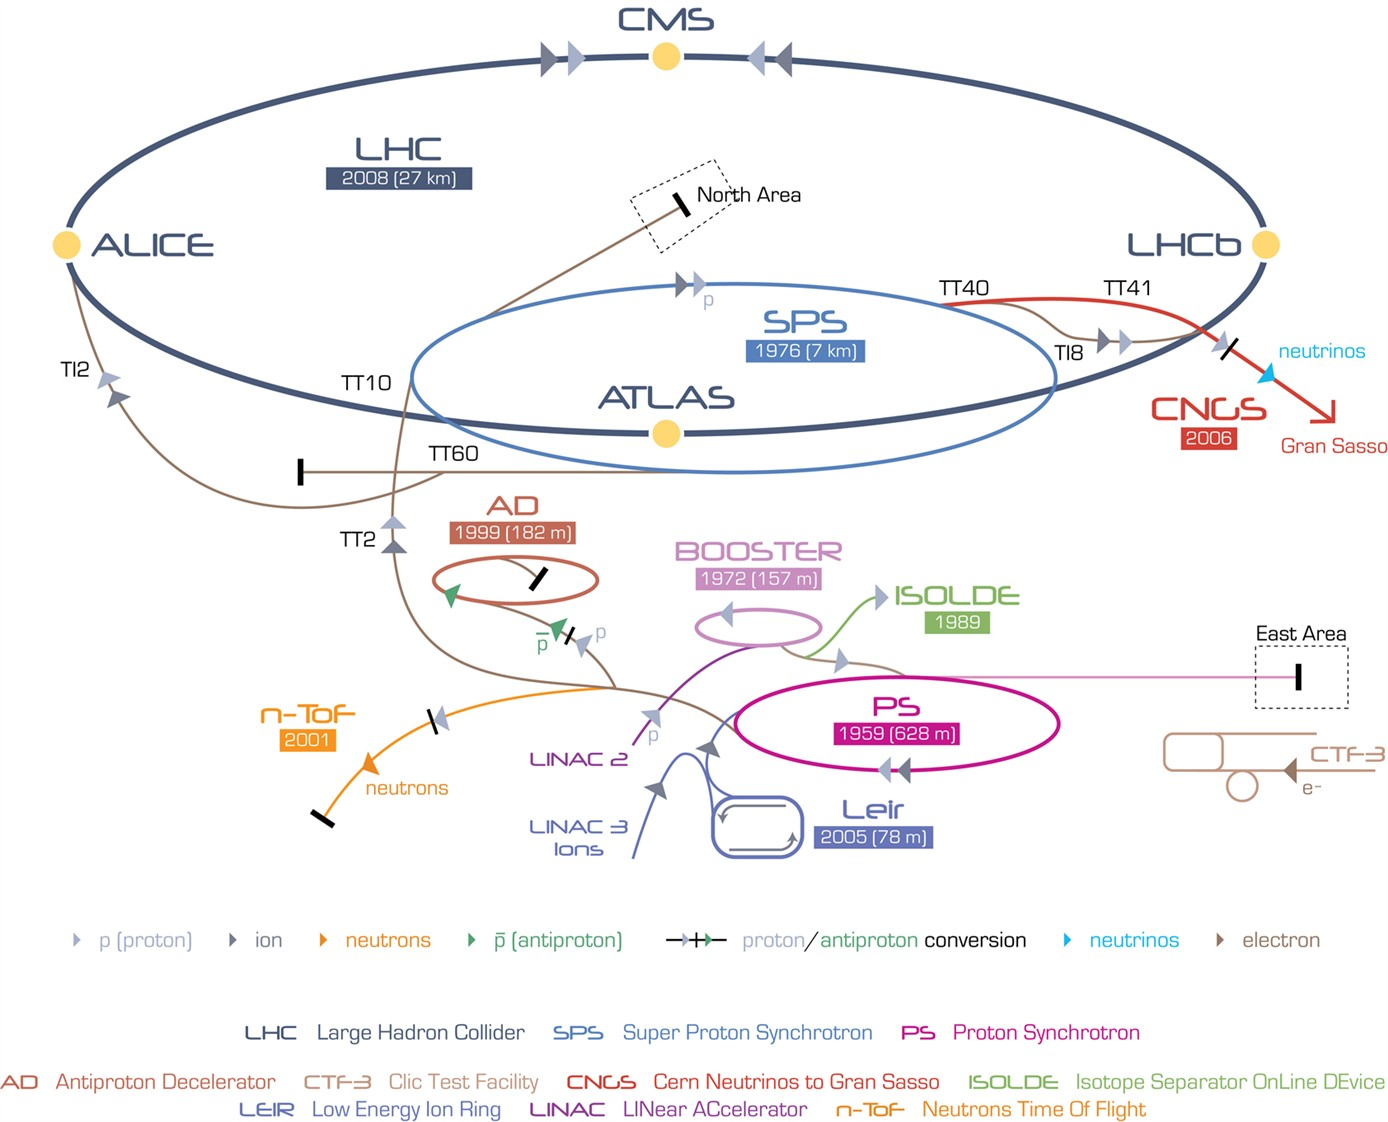
\includegraphics[width=0.8\textwidth]{detector/figures/ring.eps}}
	\caption{A schematic showing the accelerator complex at CERN. Protons are
        extracted from Hydrogen gas and injected in the first machine, the linear 
        accelerator LINAC2 that starts the acceleration chain. When protons reach
        an energy of 50~\mev\ they are injected into the Proton Synchrotron Booster
        (PSB) and accelerated up to the energy of 1.4~\gev. The second circular
        accelerator, the Proton Synchrotron (PS) brings the energy of the protons
        to 25~\gev\ previous to injecting them into the last machine before the LHC,
        the Super Proton Synchrotron (SPS). Protons of 450~\gev\ finally enter the
        LHC where they are boosted to energies of up to 4~\tev.
        The four main LHC experiments are shown on the collider ring.}
\end{center}\end{figure}

The LHC program was approved by CERN Council in 1994, followed by the approval of
the four main experiments physics programs: ATLAS~\cite{Aad:2008zzm} and CMS~\cite{cms}
in 1996; ALICE~\cite{alice} in 1997; LHCb~\cite{lhcb} in 1998.
Works towards the installation of the most powerful particle accelerator of the world
started when the Large Electron Positron Collider (LEP) was dismantled in 2000 to 
give up its place in the tunnel to the LHC, which was then fully operational by 2008.

The LHC is composed of eight arcs 2.7~km long, each of which contains 154 dipole 
magnets, whose function is to  bend the beams along the circular trajectory, and
49 quadrupole magnets, that focus the beam. These superconducting magnets operate
at a temperature of 1.9~K, maintained by means of liquid Helium vessels.
Eight insertions are placed inbetween the arches. Each insertion has a specific
role that characterizes its design and can be injection, beam dumping, beam cleaning,
or ``physics'', i.e. make the beams collide within an experiment.

First proton beams were circulated on 10th September 2008 and right on the verge of
getting the first collisions at a \cme $\rts=900\gev$ nine days later, an electrical
connection joining superconducting wires of a dipole and a quadrupole
failed. This caused the release of liquid Helium in the insulating vacuum,
resulting in an explosion that severely damaged the machine.
After more than one year devoted to repair the damage and consolidate the security,
on 30th November 2009 the LHC became the world's highest energy particle 
accelerator\footnote{\url{http://press.web.cern.ch/press/PressReleases/Releases2009/PR18.09E.html}}:
\begin{quotation}\small
Geneva, 30 November 2009. CERN's Large Hadron Collider has today become the world’s highest energy particle accelerator, having accelerated its twin beams of protons to an energy of 1.18 TeV in the early hours of the morning. This exceeds the previous world record of 0.98 TeV, which had been held by the US Fermi National Accelerator Laboratory’s Tevatron collider since 2001. It marks another important milestone on the road to first physics at the LHC in 2010.
\end{quotation}



The main performance figure of merit for an accelerator is the luminosity, the 
instantaneous luminosity $\mathcal L$ being defined as 
\begin{equation}\label{eq:lumiN}
\mathcal{L}\times\sigma=\dfrac{dN}{dt}=f\times n\dfrac{N_1\times N_2}{A}\times\sigma.
\end{equation} 
Here $dN/dt $ is the event rate of a certain process and $\sigma$ is its cross 
section. This rate is directly proportional to the the frequency $f$, the number 
of bunches $n$ and the number of particles in the two bunches $N_1, N_2$, and
inversely proportional to the beam cross-section $A$.

Integrating over the accelerator active time (a ``fill'', when stable beams are kept
colliding) gives the \textit{integrated luminosity}, relating the total number 
of produced events $N_{tot}$ to the cross-section:
\begin{equation}\label{eq:intLumi}
\int \mathcal L dt  = \dfrac{N_{tot}}{\sigma}.
\end{equation}




%http://accelconf.web.cern.ch/accelconf/IPAC2013/papers/moyab101.pdf
%http://cerncourier.com/cws/article/cern/54381

\begin{table}\centering
	\begin{tabular}{lllll}\toprule
        Parameter                       & designed      &       2010 &  2011     &   2012\\ \midrule
        Beam energy (\tev/c)            & 7             & 3.5        & 3.5       & 4    \\
        Beta function $\beta*$ (m)      & 0.55          & 2.0/3.5    & 1.5/1.0   & 0.6  \\
        Max. No. bunches/beam           & 2808          & 368        & 1380      &1380  \\
        Max. No. protons/bunch          & 1.15$\times10^{11}$ & 1.2$\times10^{11}$ & 1.45$\times10^{11}$ & 1.7$\times10^{11}$ \\
        Bunch spacing (ns)              & 25            & 150       & 75/50        & 50 \\
        Peak luminosity (\cmm2\sm1)     & 1$\times10^{34}$& 2.1$\times10^{32}$& 3.7$\times10^{33}$& 7.7$\times10^{33}$\\
        Emittance $\varepsilon_{n}$ ($\mu$rad)&3.75     &   2.0      & 2.4      & 2.5   \\
	\bottomrule\end{tabular}\caption{Overview of some parameters for the LHC performance comparing the design values with their time
        evolution during the first long run operation in 2010-2013~\cite{Lamont}.}\label{tab:lhcpar}
\end{table}

\begin{figure}[tb]\begin{center}
	\subfigure[]{\label{fig:intlumi}
  	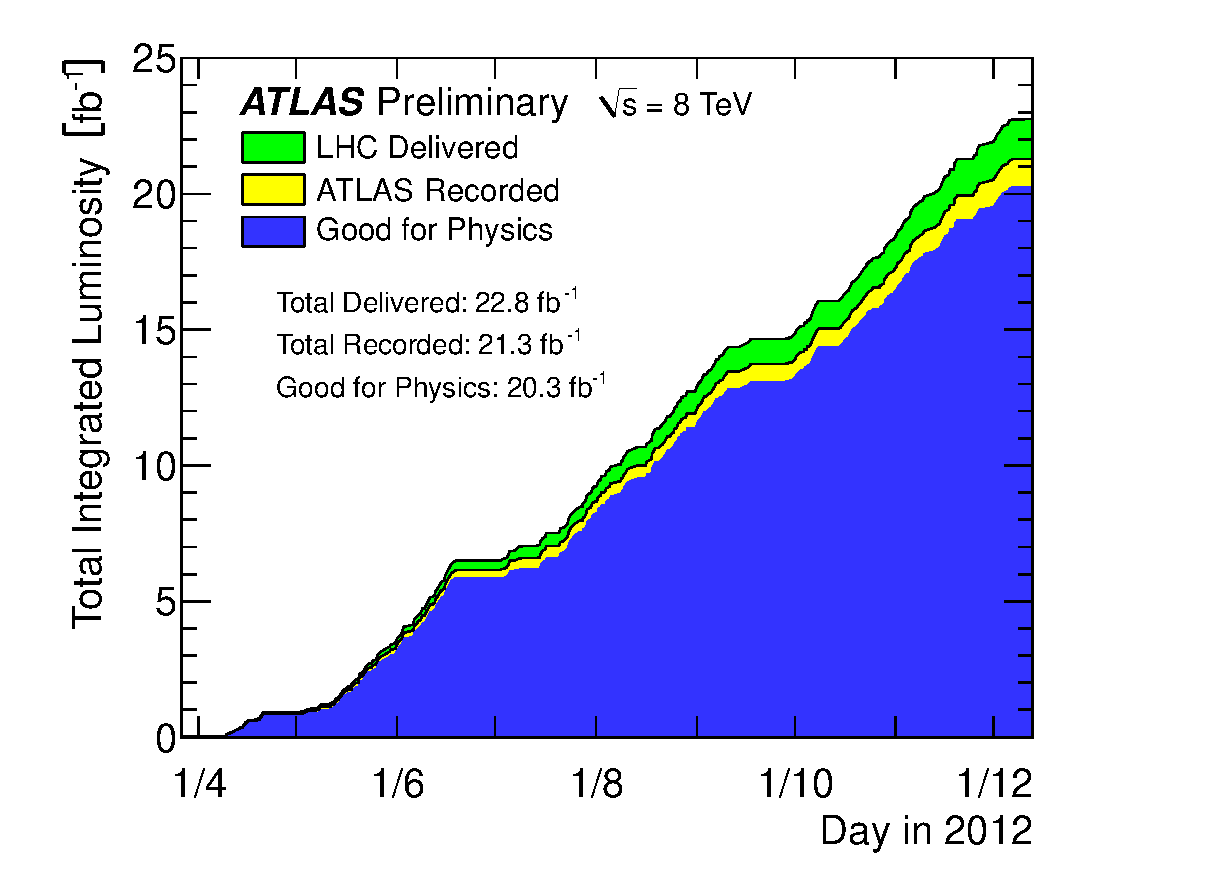
\includegraphics[width=0.48\textwidth]{detector/figures/intlumivstime2012DQ}}
	\subfigure[]{\label{fig:mu}
  	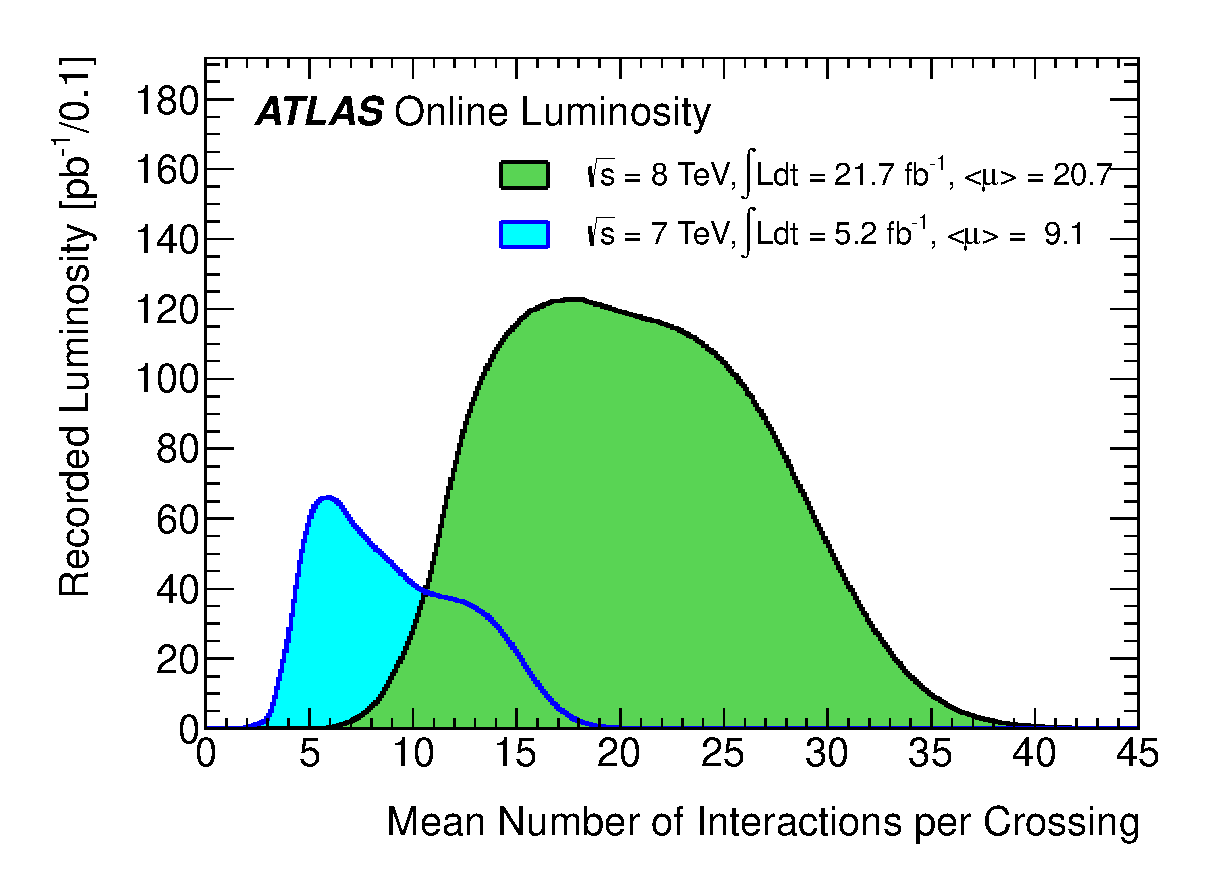
\includegraphics[width=0.48\textwidth]{detector/figures/mu_2011_2012-dec}}
	\caption{(a) Total integrated luminosity versus time delivered by the LHC to ATLAS (in green), recorded by the experiment 
        (in yellow) and selected as ``good data'' for analysis (in blue) for p-p collisions at \rts=8~\tev.
        (b) Mean number of interactions per beam crossing during 2011 and 2012 LHC runs, where 
        $\mu = \mathcal L\times \sigma_{\rm inelastic}/f$ depends on the instantaneous luminosity $\mathcal L$, the p-p inelastic
        cross section $\sigma_{\rm inelastic}$ and the revolution frequency $f$.~\cite{lumi}}
%Number of Interactions per CrossingMore details on this can be found in arXiv:1101.2185. 
\end{center}\end{figure}

In 2012 LHC reached a peak luminosity of 7.7$\times10^{33}$~\cmm2\sm1\ which is
more than half the design luminosity, as shown in Table~\ref{tab:lhcpar} together
with other parameters relevant for the accelerator performance. Over the last
year of data taking before the long shutdown\footnote{LHC terminated the p-p program
at the end of 2012, operated proton-heavy ion collisions for two months at the beginning
of 2013 and then stopped for what is called the first long shutdown. During this two-years
time the accelerator and the experiments as well will undergo substantial maintenance and 
upgrade works, in order to be re-operated in 2015 with higher performance at an higher
\cme for particle collisions.}
ATLAS collected about 20\ifb\ of p-p collision data at \rts=8~\tev.
Figure~\ref{fig:intlumi} shows the delivered luminosity from the start of stable beams until beam dump and the luminosity recorded by
ATLAS during stable beam conditions, the difference with respect to the delivered luminosity being due to Data AQuisition (DAQ)
inefficiencies. Of the recorded luminosity, only a part is usable for analysis, and is what is called ``good data'', i.e. 
the data that satisfy Data Quality (DQ) requirements assessed after reprocessing.

In order to increase the luminosity LHC operates with higher number of protons per bunch as well as higher
 number of bunches per beam and reduces the inter-bunch latency time.
This overall defines a set of challenges that physics analysis will face associated to the high luminosity.
Even at the detector design stage, the high frequency of collision environment foreseen influenced
the choice of radiation resistance material for the experiment sub-systems. Concerning directly the physics
instead we can list the main problematics as being \textit{underlying events} and \textit{pile-up}

Underlying events are the product of the hadronic character of p-p hard interaction, where the main collision process
is accompanied by secondary parton interactions at low transfered momentum (soft QCD) and are flavor- and color-connected to the
hard scattering. They are observed as jets of particles close to the direction of the beam and are in general not 
separable from the event of interest. Their contribution can be studied with Monte Carlo techniques tuned with data from 
\textit{minimum bias} events, as perturbative theory does not properly model low momentum QCD.
%%%%%%%%%%AAAAAAAAAAAAAAAAA


Pile-up events are distinguished between \textit{in-time} and \textit{out-of-time} pile-up. The first ones come 
from the multiple inelastic scatterings of protons in the same bunch, as if we consider a cross-section of 80~mb
at the nominal luminosity of $10^{34}$~\cmm2\sm1 the number of events per second will be something like
a billion. This translate, at a collision frequency of one crossing every 25~ns, to about 20 interactions per
crossing that will be detected simultaneously. On the other hand, the inter-bunch time interval is so short
that the electronics reading the detector might not keep up with the frequency of collisions, leading to the
cumulation of events that happened in different beam crossings.

ATLAS makes use of a three-level trigger system (described in Section~\ref{sec:trigger}) to identify
and record only the events of interest, while the pile-up issues are dealt with at the analysis 
reconstruction level.



\section{The ATLAS detector}\label{sec:atlas}

ATLAS (A Toroidal LHC ApparatuS)~\cite{Aad:2008zzm} is a general purpose experiment
aimed at exploring a vast range of physics scenarios. It is characterized by
a full coverage of the space around the p-p interaction point and complete
containment of the particles produced in the collision. Different subsystems are
layered concentrically one after the other, each of them pursuing a specific task. 
Right around the interaction point
(IP) where the LHC makes protons collide there is the Vertex Detector, reconstructing
charged particles trajectories that are bended by the first solenoid magnet surrounding
the Vertex Detector. Particles going through it then encounter the two calorimeter systems,
the Electromagnetic and the Hadronic one. Muons are the only particles that will pass
the calorimeters material (beyond neutrinos) and a dedicated Muon Spectrometer is the last
piece of detector, embedded in a huge toroidal magnet. The detector complex is presented
as a schematic in Figure~\ref{fig:atlas}. 

\begin{figure}[tb]\begin{center}
	\subfigure{\label{fig:atlas}
  	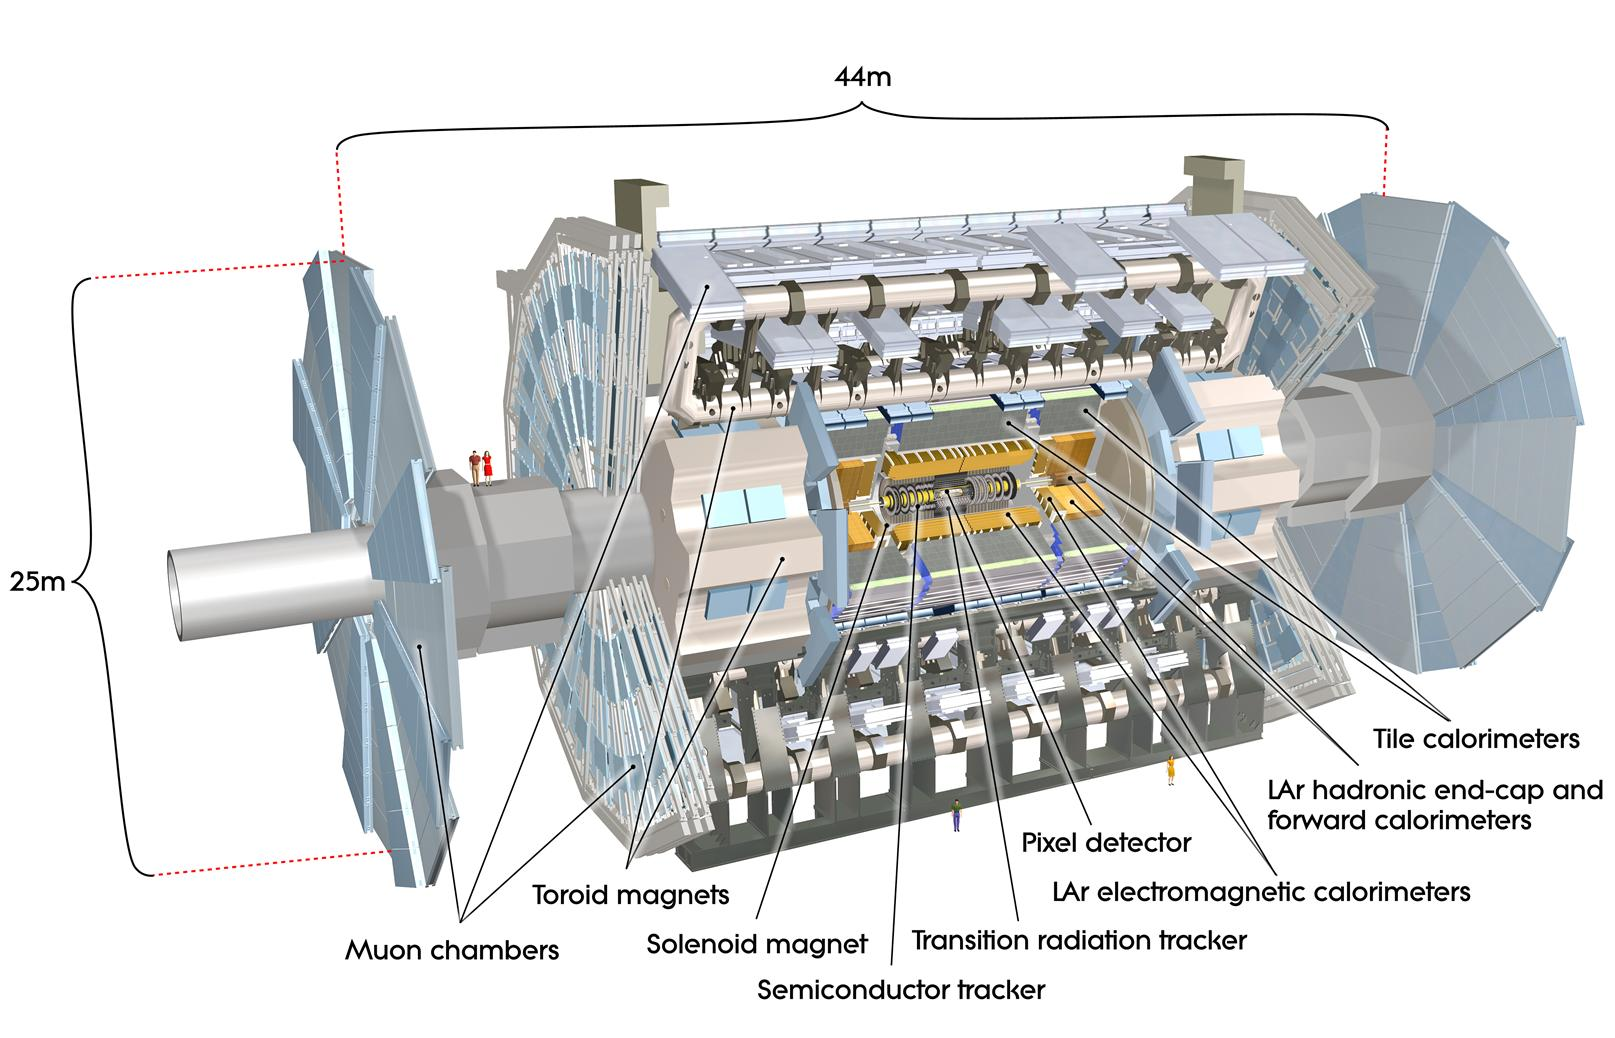
\includegraphics[width=0.9\textwidth]{detector/figures/atlas}}
	\caption{Schematic drawing of the ATLAS experiment. The detector subsystem are indicated as well as the total dimensions.}
\end{center}\end{figure}

\subsection{Coordinate system}

Protons from the two circulating beams are made to collide in the center of the ATLAS detector, in the region
that takes the name of Interaction Point (IP). The IP is taken as the origin of a three dimensional XYZ right-handed
coordinate system. The Z axis is tangent to the trajectory of the beams while the XY plane is perpendicular to
it and defines a symmetry plane for the detector, dividing it into the $A$ and $C$ sectors, respectively in the
positive and negative Z semi-axes. Figure~\ref{fig:coord} shows a schematic of the coordinate system.

\begin{figure}[tb]\begin{center}
	\subfigure[]{\label{fig:coord}
  	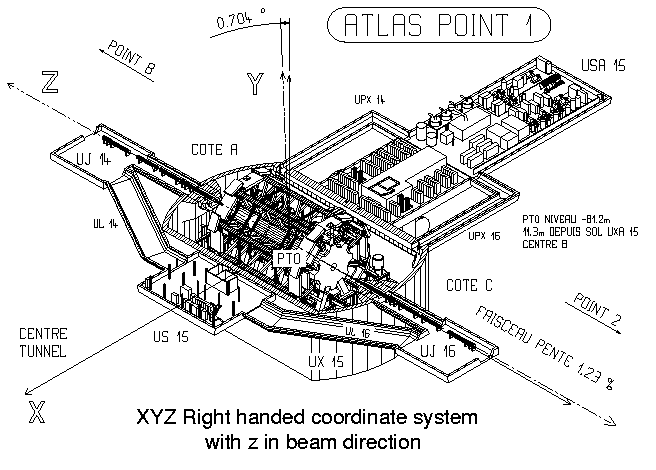
\includegraphics[width=0.6\textwidth]{detector/figures/coord}}\hskip3ex
        \subfigure[]{\label{fig:spherical}
  	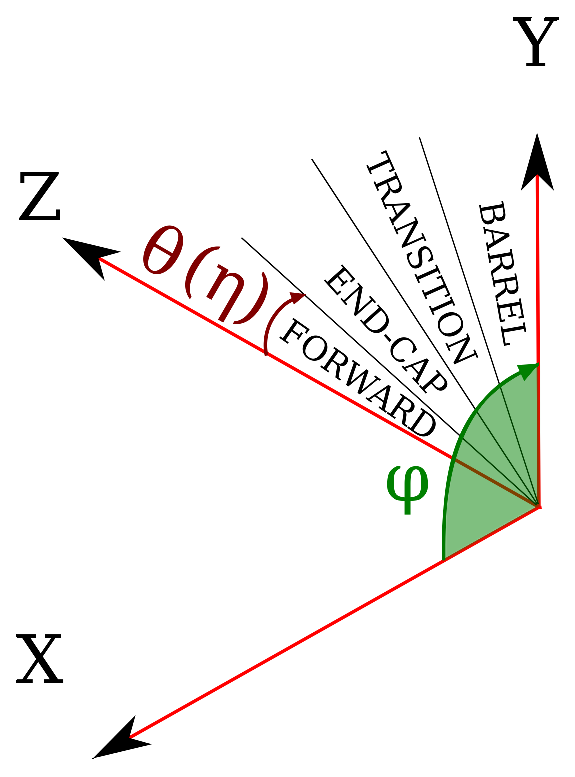
\includegraphics[width=0.3\textwidth]{detector/figures/spherical}}
	\caption{(a) Drawing of the ATLAS experiment with the cartesian coordinate system. The positive X axis points towards the center of the LHC
        ring. The positive Z axis points todards the circulating direction of beam 2. (b) Simple schematic showing the spherical coordinates and the
        region definition in terms of the absolute value of the pseudorapidity $\eta$. These regions are symmetrical with respect to the transverse
        XY plane.}
\end{center}\end{figure}

In terms of polar coordinates, the Z axis is again along the beam axis and in the transverse plane 
the $R$ and $\phi$ coordinates are defined with $\phi$ ranging between 
$-\pi$ and $+\pi$ with respect to the X axis. In terms or spherical coordinates (see Figure~\ref{fig:spherical}),
the radial vector $R$ originates from the IP,  the azimuth $\phi$
is the same as the polar angle $\phi$, 
and the polar angle $\theta$ is measured with respect to the Z axis and
ranges between 0 and $\pi$. 

Since the interaction initial energy is unknown, being dependent on the parton distribution functions for the proton
energy, it is useful to define the transverse component of variables of 
interest\footnote{These quantities transverse initial value will be, indeed, zero, as the protons are accelerated along the Z axis.}  
like the energy and the momentum, being taken as the projection on the XY plane:

\begin{equation}\label{eq:transv}
\et = E\sin\theta, \qquad \pt = p\sin\theta.
	\end{equation}

Another common variable used at hadron colliders to describe the polar distribution and preferred to the simple
polar angle $\theta$ is the pseudorapidity $\eta$:
\begin{equation}\label{eq:pseudorapidity}
        \eta \equiv -\ln\bigg(\tan\frac{\theta}{2}\bigg);
	\end{equation}
which, for relativistic regimes, is equal to the rapidity $y$:
\begin{equation}\label{eq:rapidity}
y \equiv \frac{1}{2} \ln \bigg(\frac{E+p_{Z}}{E-p_{Z}}\bigg);
	\end{equation}
and $\Delta y$ and $\Delta \eta$ are Lorentz invariant. The pseudorapidity is preferred
to the rapidity as it does not require knowing the particle mass but only its polar position.
The distance between two particles is often referred to in terms of $\Delta R$:
\begin{equation}\label{eq:deltar}
\Delta R = \sqrt{\Delta^{2}\eta + \Delta^{2}\phi}.
	\end{equation}


%since particles produced in collisions are not uniformely distributed in $\theta$. 
Figure~\ref{fig:spherical} shows how different pseudorapidity regions are named. Particles
along the Z axis have a pseudorapidity $|\eta|=\infty$, particles along the Y axis have
a pseudorapidity $|\eta|=0$. ATLAS has an excellent hermeticity and is able to cover 
pseudorapity regions up to $|\eta|=4.9$. Typically, physics analysis consider objects in
the pseudorapity region  $|\eta|<2.5$. For a quick visualization of the correspondence
in terms of polar angle distribution, some pseudorapidity values are reported in Table~\ref{tab:etatheta}.
%AAAAAAAAAAAAAAAAA add barrel forward blabla exact def


\begin{table}[htb]\centering\begin{tabular}{cccccccccc}\toprule
$\theta$ & 0$^{\circ}$ & 5$^{\circ}$ & 10$^{\circ}$ & 20$^{\circ}$ & 30$^{\circ}$ & 45$^{\circ}$ & 60$^{\circ}$ & 80$^{\circ}$ & 90$^{\circ}$ \\
$\eta$ & $\infty$ & 3.13 & 2.44 & 1.74 & 1.31 & 0.88 & 0.55 & 0.175 & 0\\\bottomrule \end{tabular}
\caption{Pseudorapidity vs polar angle values.}\label{tab:etatheta}\end{table}

\subsection{Magnets}\label{sec:magnets}

ATLAS is provided with four superconducting magnets that allow the measurement of
charged particles momenta by curving their trajectory. 

A central solenoid sits 
around the inner detector and produces a 2~T magnetic field along the direction
parallel to the beam axis. It is only 45~mm thick (equivalent to 0.66 radiation lenghts $X_0$)
and is cooled with liquid Helium, sharing the cryostat with the electromagnetic calorimeter.

Three toroidal magnets, one in the barrel region and the other two in the end-cap regions,
produce a magnetic field of 0.5~T and 1~T respectively in the direction orthogonal to the muons trajectory.

\subsection{Inner detector}\label{sec:innerdet}

The Inner Detector (ID) is the subsystem closest to the IP and tracking charged particles arising from collisions allows for 
the measurement of their momentum and vertex reconstruction with excellent resolution. At the design choices level, radiation resistance had to
be taken into account, as well as reducing the amount of material to be placed in front of the calorimeters to avoid spoiling the energy measurement.
This quantity varies between 0.5 and 2.5~$X_0$ depending on the pseudorapidity region, most of it coming from supporting equipment. This material
is responsible for photon conversions and electron bremsstrahlung.

The ID is surrounded by the central solenoid magnet (Section~\ref{sec:magnets}) and is composed by three subsystems, 
from the closest to the furthest from the IP: a pixel detector, a silicon strip detector and
a straw detector (Figures~\ref{fig:innerdet1} and~\ref{fig:innerdet2}).

\begin{figure}[tb]\begin{center}
	\subfigure[]{\label{fig:innerdet1}
  	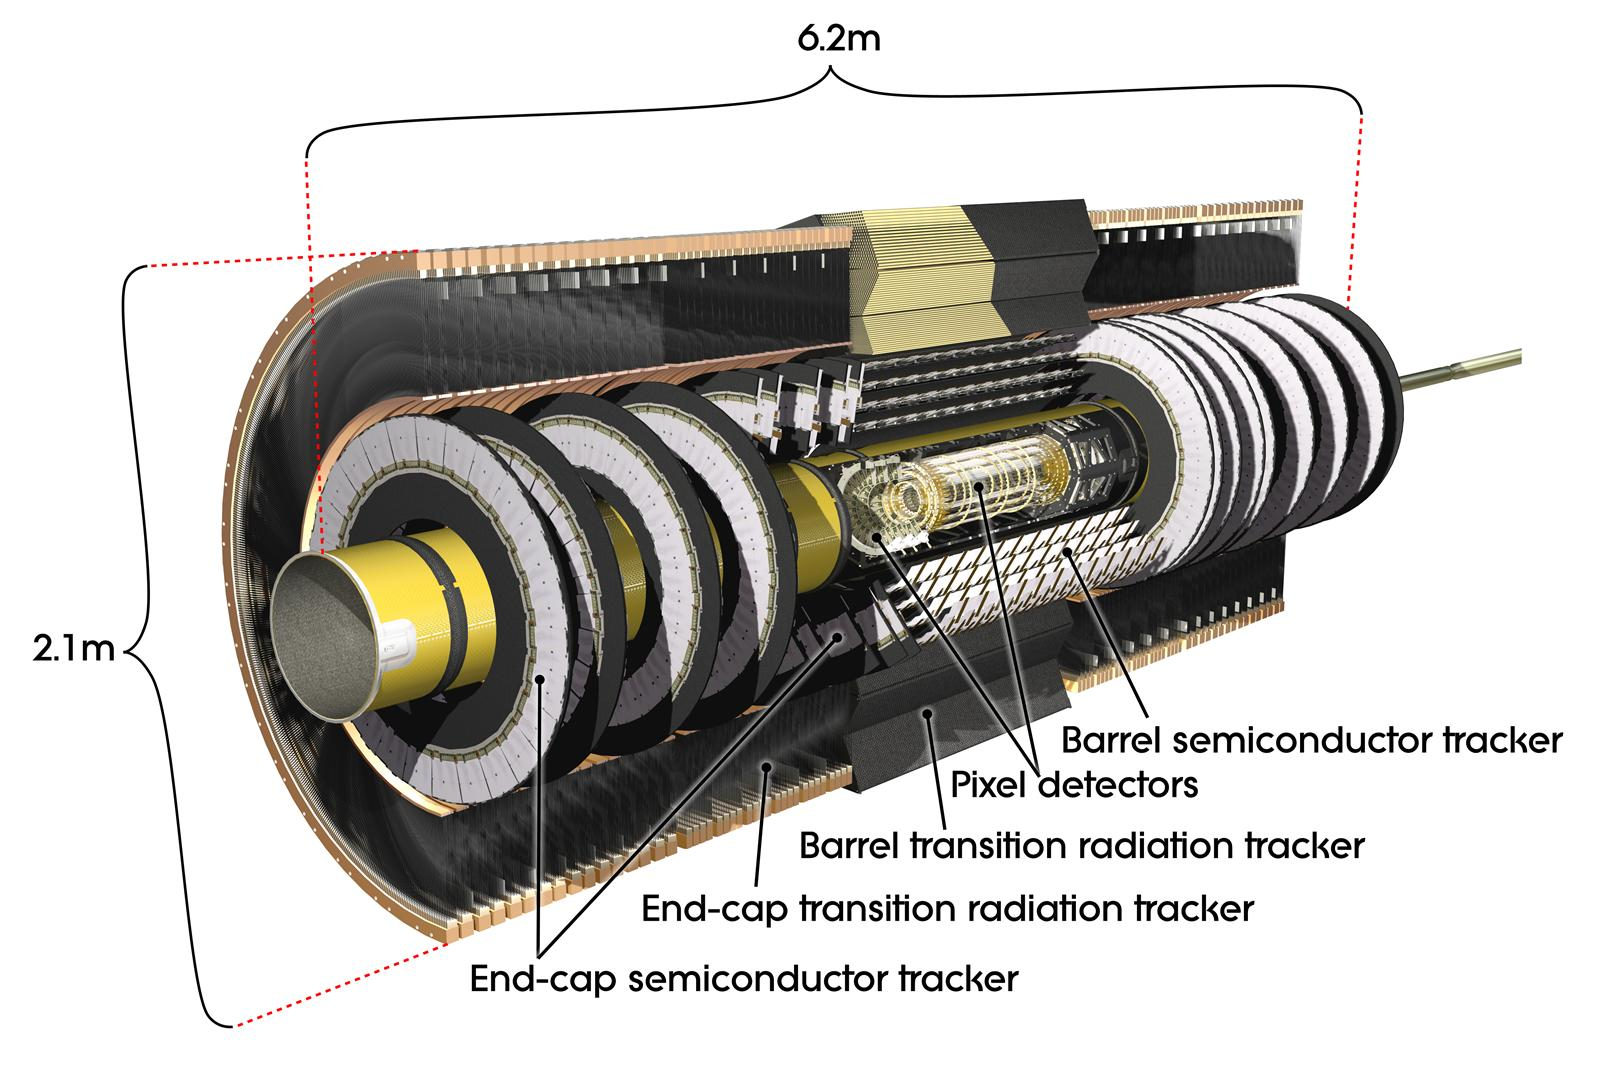
\includegraphics[width=0.6\textwidth]{detector/figures/innerdet}}
	\subfigure[]{\label{fig:innerdet2}
  	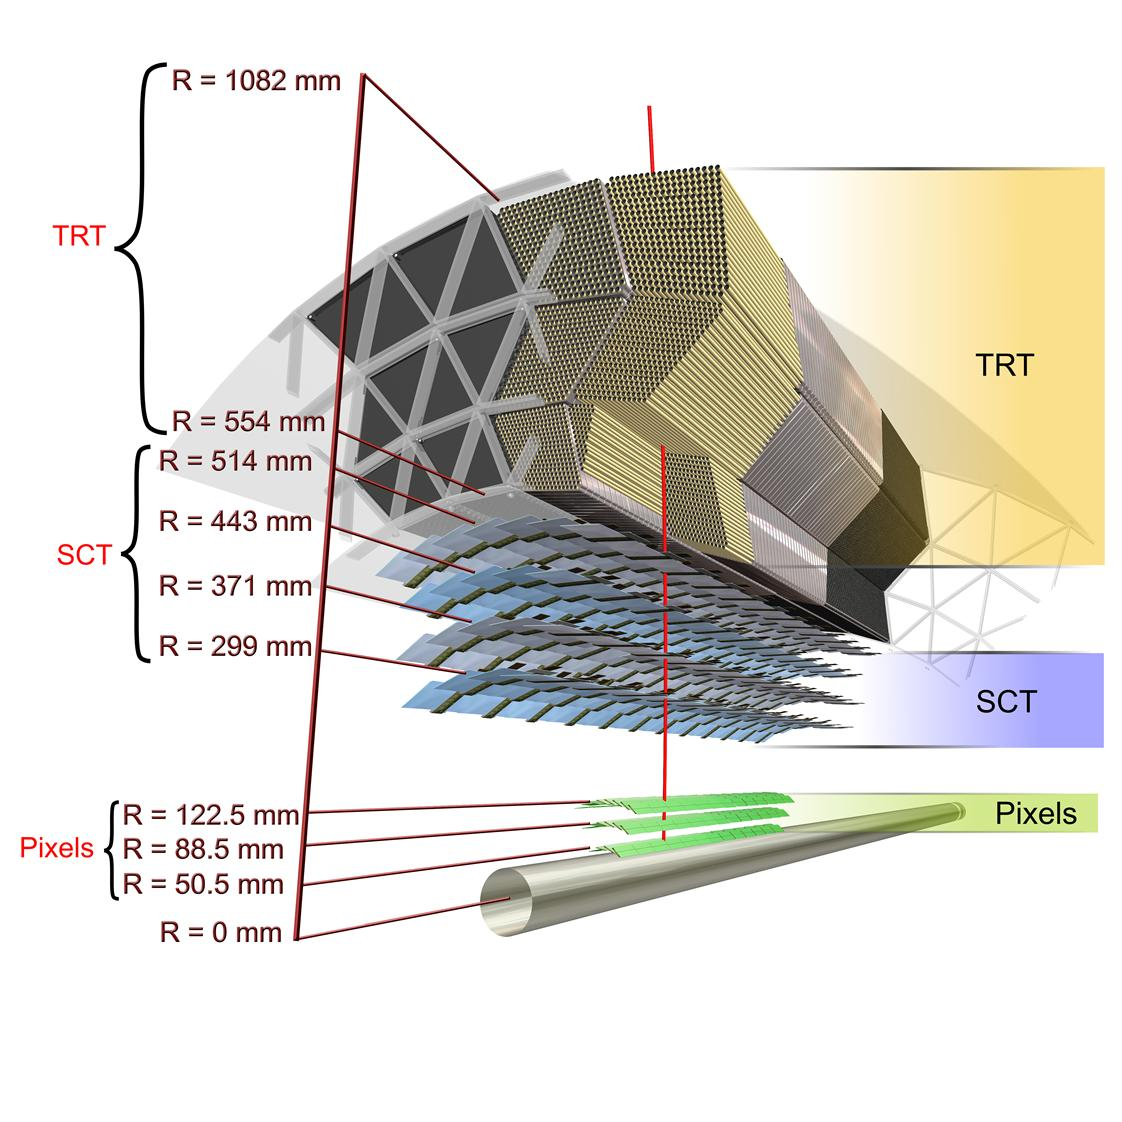
\includegraphics[width=0.37\textwidth]{detector/figures/innerSection}}
	\caption{(a) Schematic of the ID system. (b) Detailed schematic of the barrel section of the ID showing the
        three subsystems and reporting the distance to the center of the beam pipe.}
\end{center}\end{figure}


\subsubsection{Silicon Detectors}

The first subsystem covers the region $|\eta|<2.5$ and  is composed by three cylindrical layers in the barrel region, each of them distant from the beam by
50.5~mm, 88.5~mm and 122.5~mm respectively, and by three concentric discs in the end-cap region, each of them distant from the beam by
49.5~mm, 58.0~mm and 65.0~mm respectively.
Each silicon pixel has a size of 50$\times$400~$\mu$m$^{2}$ and is 250~$\mu$m thick, 
with in total $\sim$80.4 million readout channels to achieve a very fine granularity.
The precision is of 10~$\mu$m in $R\phi$ and 115~$\mu$m in Z and $R$ in the barrel and end-cap
region respectively.

The very first layer is called $B-$layer as, thanks to its position really close to the IP,
allows for the reconstruction of secondary vertices associated with the production of
 short lived particles such as $B-$hadrons. This information is very useful to identify
particle jets from $b$ quarks\footnote{The $b-$tagging technique will be discussed in %AAAAAAAAAAAAAAAAAAAA
}.

After the three layers of pixel detectors, come four layers of  silicon strip detectors. The SemiConductor
Tracker (SCT) also covers the region $|\eta|<2.5$ with a barrel and end-cap design similar to the 
pixel detector one, being composed by eight silicon bands (two per layer) 128~mm long and 80~$\mu$m large.
It makes use of $\sim$6.3 millions readout channels and the resolution achieved is of 17~$\mu$m 
in $R\phi$  and 580~$\mu$m in Z and $R$ in the barrel and end-cap region respectively.

By allowing for four redundant position measurements\footnote{One of the coupled layers is rotated of $40$mrad with respect
to the other, which is parallel to the axis, giving a small stereo angle for a redundancy in the $\phi$ coordinate measurement.}, 
the SCT contributes mainly to the momentum reconstruction.

%Silicon has a band gap of just 3.6 eV, that is the minimum energy to create an electron/hole pair. Thus a minimum ionising particle creates around 80 electron/hole pairs per $\mu$m through primary and secondary ionisation.

\subsubsection{Transition Radiation Tracker}

In order to reduce the amount of material in front of the calorimeters, and to reduce the construction costs as well,
in the third subsystem the semiconductor technology has been substituted with straw detectors.
The Transition Radiation Tracker (TRT) consists of thin proportional chambers made of straw polyimide drift tubes, 4~mm in diameter.
The drift tubes are filled with a gas mixture composed of: 70\% Xenon, 27\% Carbon Dyoxide, 3\% Oxygen. The anode 
collecting the electrons from the ionized gas at the passage of the charged particle is made of
tungsten covered in gold.

In the barrel region the tubes are 144~cm long and placed parallel to the beam axis, while in the 
end-cap region they are 37~cm long and positioned radially in wheels, with layers of radiator foils alternated 
to layers of straws. The resolution achieved is of 130~$\mu$m in $R\phi$ and Z$\phi$  in the two regions respectively.
The covered pseudorapidity region is of $|\eta|<2.0$ and the readout is composed by $\sim$351000 channels.

About 36 measurements per track are taken, and since each channel provides two independent thresholds per hit,
it is possible to discriminate between electrons and pions, since the firsts will more probably reach the
high threshold.

In the end, the combination of the three ID subsystems gives very precise $R\phi$ and Z measurements, as well as good track pattern recognition.
The resolution on the transverse momentum, measured with cosmic muon calibration runs~\cite{id_cosmic}, is:

\begin{equation}\label{eq:momentumres}
\frac{\sigma_{\pt}}{\pt}=P_1 \oplus P_2 \times \pt,
	\end{equation}
where $P_1=1.6\pm0.1\%$ and $P_2=(53\pm2)\times10^{-5}$~\GeV$^{-1}$. This means a 
resolution of~$\sim$1.6\% for tracks with $\pt\sim$1~\GeV\ and 
$\sim$50\% for tracks with $\pt\sim$1~\tev.


\subsection{Calorimeters}\label{sec:calo}

Particles leaving the ID and surviving the crossing of the central solenoid magnet
will face the calorimeter system, depicted in Figure~\ref{fig:calorimeters}.
Different technologies are used in the barrel and end-cap regions for both the
Electromagnetic and the Hadronic calorimeters.

\begin{figure}[tb]\begin{center}
	\subfigure{\label{fig:calorimeters}
  	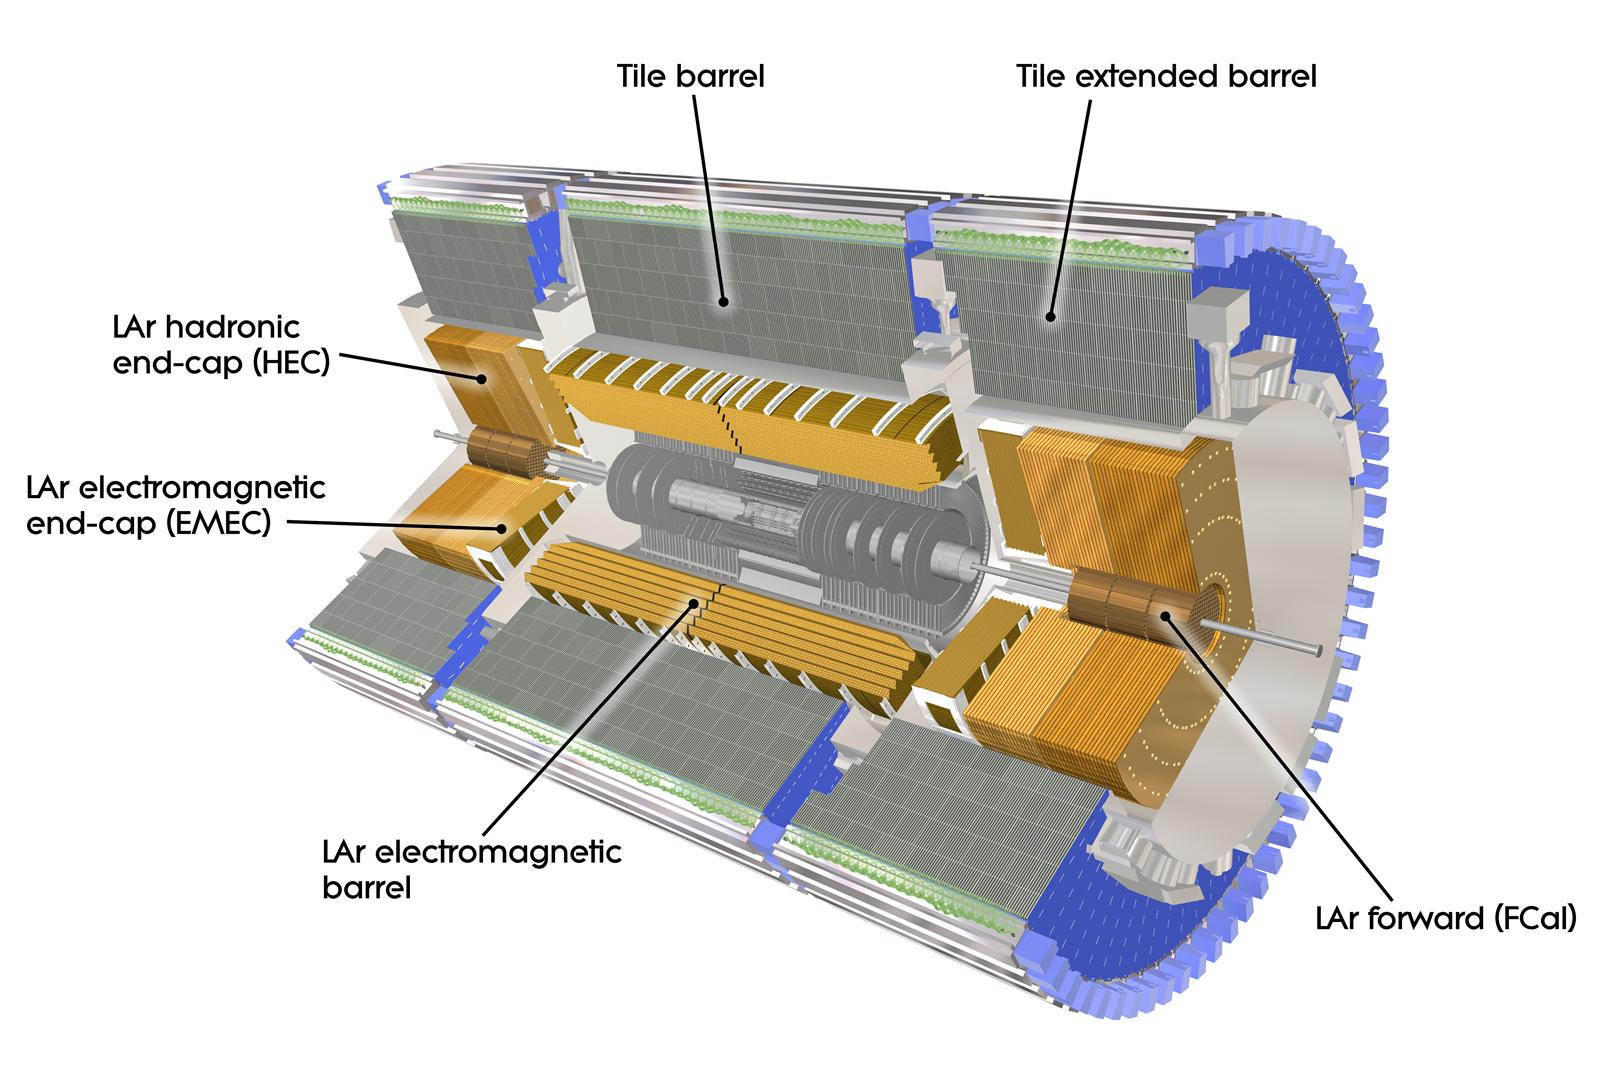
\includegraphics[width=0.8\textwidth]{detector/figures/caloBarrel}}
	\caption{Schematic of the calorimeter complex of the ATLAS detector.}
\end{center}\end{figure}

\begin{figure}[tb]\begin{center}
	\subfigure[]{\label{fig:calolar}
  	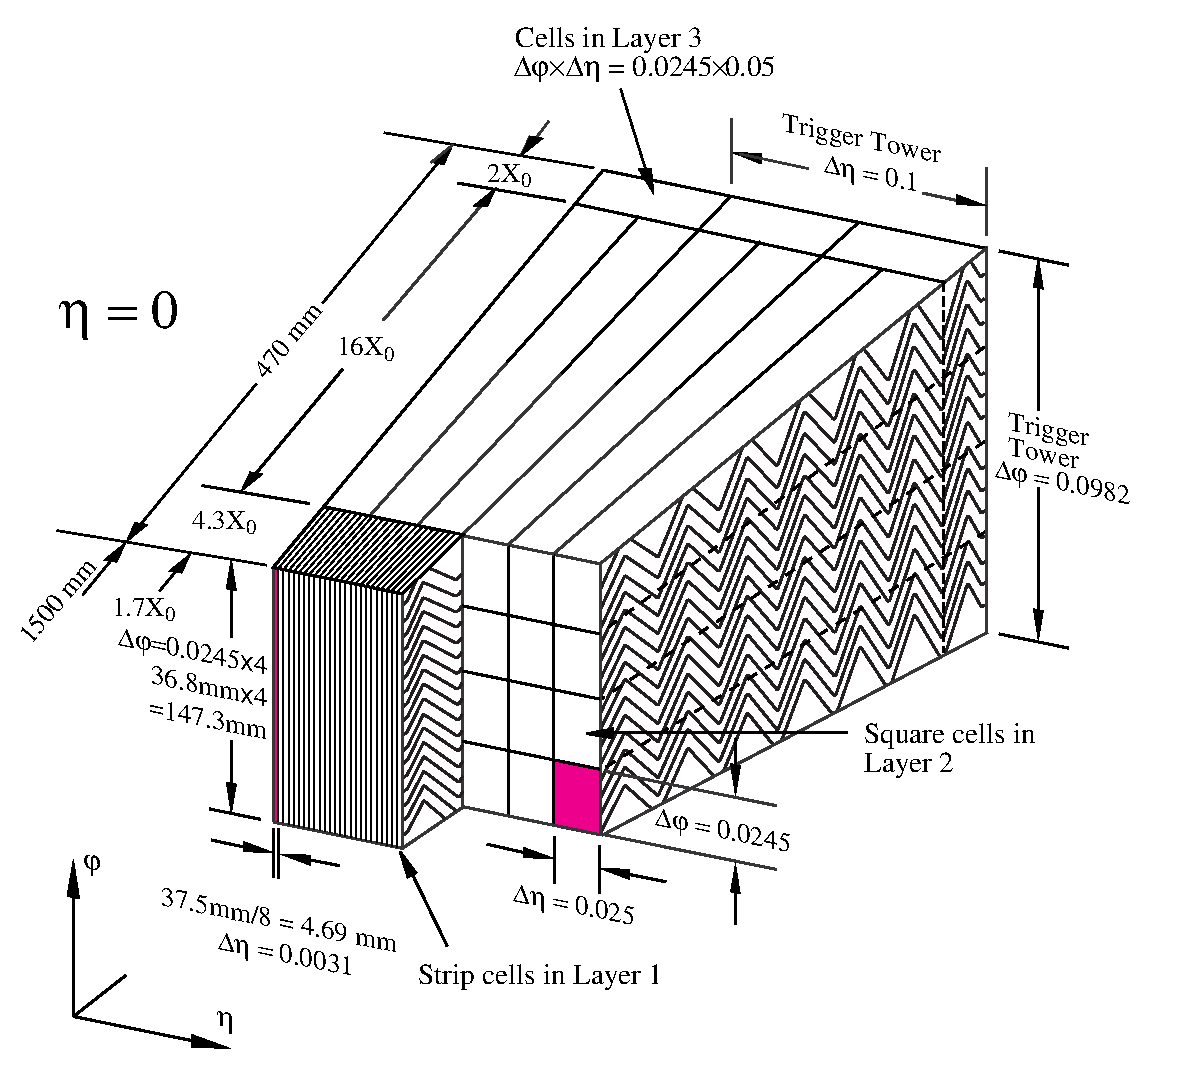
\includegraphics[width=0.48\textwidth]{detector/figures/caloLAr2}}
	\subfigure[]{\label{fig:calotile}
  	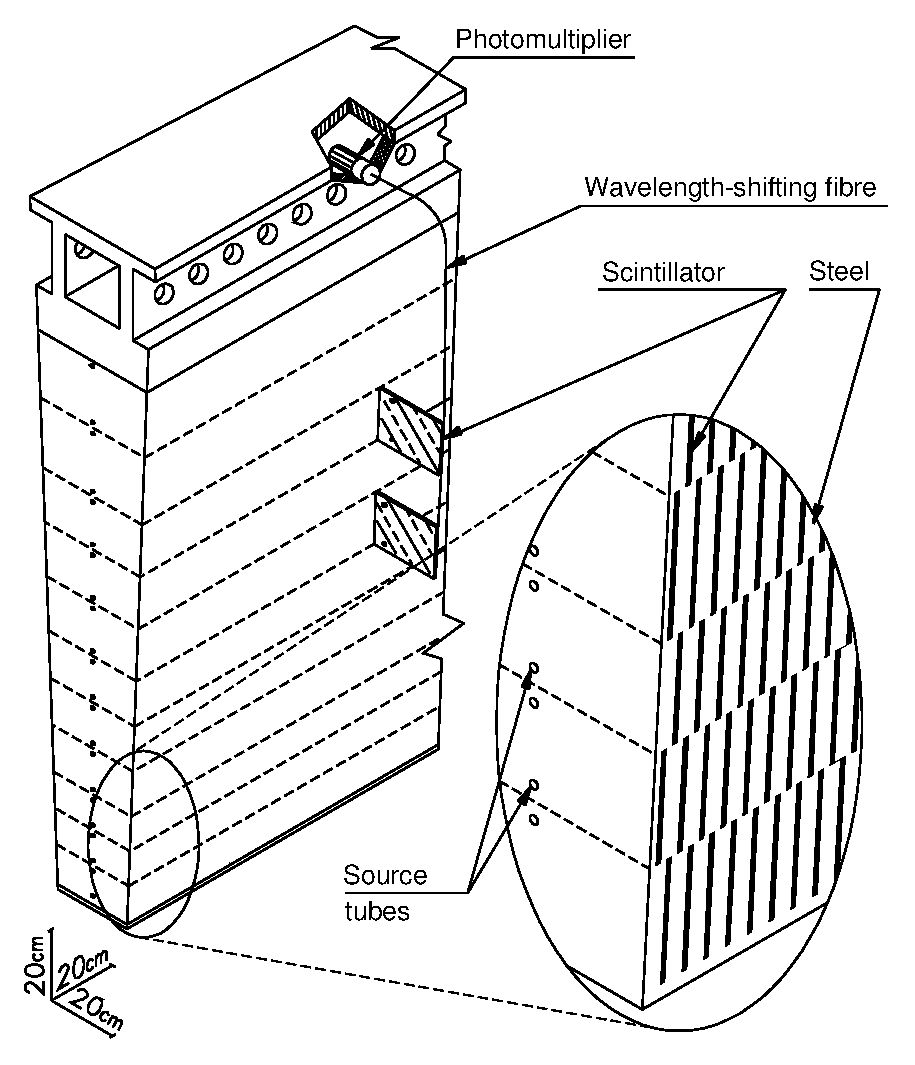
\includegraphics[width=0.38\textwidth]{detector/figures/caloTile}}
	\caption{(a) Schematic drawing of a module of the Electromagnetic barrel calorimeter. 
        (b) Schematic drawing of a module of the Hadronic barrel calorimeter.}
\end{center}\end{figure}


\subsection{Muon spectrometer}\label{sec:muonspec}

\subsection{Trigger system}\label{sec:trigger}

